\chapter{背景}

\section{极大似然估计(maximum likelihood estimation)}

给定概率分布$D$,已知其概率密度函数(连续分布)或者概率质量函数(离散分布)为$f_D$,
以及一个分布参数$\theta$,我们可以从这个分布中抽一个具有$n$个值的采样$X_1,X_2,\cdots,X_n$,利用
$f_D$计算出其似然函数
\begin{equation}
    L(\theta|x_1,\cdots,x_n)=f_\theta(x_1,\cdots,x_n)
\end{equation}

若$D$是离散分布,$f_\theta$即是在参数为$\theta$时观测到这一采样的概率;
若其是连续分布,$f_\theta$则为$X_1,X_2,\cdots,X_n$联合分布的概率密度函数
在观测值处的取值。

从数学上来说,我们可以在$\displaystyle \theta$的所有可能取值中寻找一个值使得似然函数取到最大值。这个使可能性最大的
$\displaystyle {\widehat {\theta }}$值即称为$\displaystyle \theta$的最大似然估计。由定义,最大似然估计是样本的函数。

\subsection*{相对熵}

最大似然估计可以从相对熵推导而来。相对熵衡量了使用一个给定分布$Q$来近似另一个分布
$P$时的信息损失,对于离散随机变量
\begin{equation}
    D_{KL}(P||Q)=\sum_{i}P(i)log\frac{P(i)}{Q(i)}
\end{equation}

其中$P$是真实分布,$Q$是近似分布。在最大似然估计的情景下,假设分布拥有一系列参数$\theta$,
我们希望通过样本得到参数的估计值$\hat{\theta}$,我们可以利用相对熵来评估估计的好坏
\begin{equation}
    D_{KL}(p_\theta(x)||p_{\hat{\theta}}(x))=\sum_{x\in E}p_\theta(x)log \frac{p_\theta(x)}{p_{\hat{\theta}}(x)}
\end{equation}

根据数学期望的定义,上式可以改写
\begin{equation}
    D_{KL}(p_\theta(x)||p_{\hat{\theta}}(x))=\mathbb{E}_\theta[log(\frac{p_\theta(x)}{p_{\hat{\theta}}(x)})]
    =\mathbb{E}_\theta[log\ p_\theta(x)]-\mathbb{E}_\theta[log\ p_{\hat{\theta}}(x)]
\end{equation}

KL值越大,参数估计越坏,因此,需要通过改变估计参数$\hat{\theta}$的值来获得最小的值,所对应的参数极为最佳估计参数
\begin{equation}
    \hat{\theta}_{best}=arg\ \min\limits_{\hat{\theta}}\ D_{KL}(p_\theta(x)||p_{\hat{\theta}}(x))
\end{equation}

假设有$n$个样本,根据\textsl{大数定律},
\begin{equation}
    \mathbb{E}_{\theta}[log\ p_{\hat{\theta}(x)}]\rightsquigarrow \frac{1}{n}\sum\limits_{i=1}^{n}log\ p_{\hat{\theta}}(x)
\end{equation}

因此我们可以通过下式去估计
\begin{equation}
    D_{KL}(p_{\theta}(x)||p_{\hat{\theta}}(x))=\mathbb{E}_{\theta}[log\ p_{\theta}(x)]-\frac{1}{n}\sum\limits_{i=1}^{n}log\ p_{\hat{\theta}}(x_i)
\end{equation}

对于一个已知的分布,其参数$\theta$是确定的。因此,$\mathbb{E}_{\theta}[log\ p_{\hat{\theta}(x)}]$为常数。因此,我们可以通过最小化KL值获得最佳估计参数:

\begin{equation}
    \hat{\theta}=arg\ \min\limits_{\theta}\ \mathbb{E}_{\theta}[log\ p_{\hat{\theta}(x)}]-\frac{1}{n}\sum\limits_{i=1}^{n}log\ p_{\hat{\theta}}(x_i)
\end{equation}

只要求和项最大,那么整体就最小,这个优化问题等价于
\begin{equation}
    \begin{aligned}
        & arg\ \max\limits_{\theta}\ \frac{1}{n}\sum\limits_{i=1}^{n}log\ p_{\hat{\theta}}(x_i)\\
        & \Rightarrow arg\ \max\limits_{\theta}\ log[\prod\limits_{i=1}^{n}p_{\hat{\theta}}(x_i)]\\
        & \Rightarrow arg\ \max\limits_{\theta}\ \prod\limits_{i=1}^{n}p_{\hat{\theta}}(x_i)
    \end{aligned}
\end{equation}

因此,要得到最佳参数估计值,只需要最大化$\prod\limits_{i=1}^{n}p_{\hat{\theta}}(x_i)$,这就是最大似然函数。

\section{频率派 vs. 贝叶斯派}

频率派和贝叶斯派的区别是是否允许先验估计。
\begin{figure}[H]
    \centering
    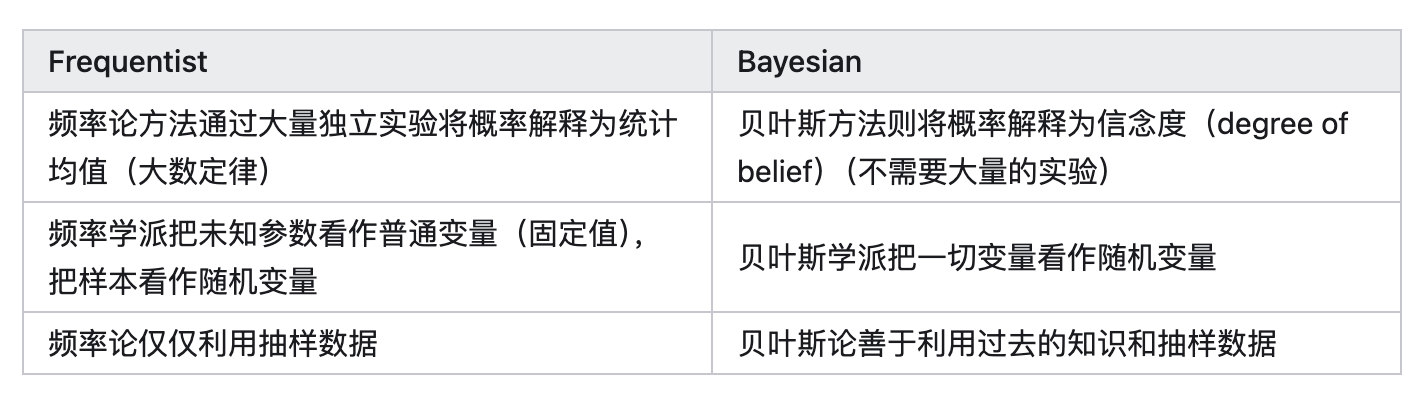
\includegraphics[scale=0.3]{figures/频率派和贝叶斯派.png}
    \caption{频率派和贝叶斯派}
\end{figure}



